%%%%%%%%%%%%%%%%%%%%%%%%%%%%%%%%%%%%%%%%%%%%%%%%%%%%%%%%%%%%%%%%%%%


\documentclass[runningheads,a4paper]{llncs}
\usepackage{graphicx}
\usepackage{amssymb}
\usepackage{amsmath}
\setcounter{tocdepth}{3}
\usepackage{graphicx}
\usepackage{clrscode}
\usepackage{url}
\newcommand{\keywords}[1]{\par\addvspace\baselineskip
\noindent\keywordname\enspace\ignorespaces#1}
\makeatletter
    \newcommand\fcaption{\def\@captype{figure}\caption}
\makeatother
\begin{document}

\mainmatter
\title{Fusing Human Faces}
\author{Xianxiang Wang}
\institute{University of Science and Technology of China, 230031 Hefei, China\\
\url{kowo@mail.ustc.edu.cn}}
%\toctitle{Lecture Notes in Computer Science}
%\tocauthor{Authors' Instructions}
\maketitle


\begin{abstract}
Face fusion technology grows more important in recent years. In this paper, we propose an algorithm to fuse features of source face into target face. There are two main challenges in our task. The first challenge is how to rearrange facial features of target face properly according to source face. The second challenge is to keep facial hues and illumination information of target face as much as possible so that output face looks more photorealistic. Our algorithm contains two steps. First, we align two faces according to facial landmarks, which give us size, location and distribution  of features of two faces, segment two faces into several triangles using Delaunay triangulation and warp the corresponding triangles of two faces into the same shape. Second, we reconstruct gradients for new face that we are going to generate. With one face image as target image and reconstructed gradients, we generate fused face by seamless clone. We propose an algorithm to reconstruct the new face gradients by preserving the weaker gradients of the target face. Our experiments show that proposed method preserves lots of illumination information and facial hues of target faces, which means output faces look more photorealistic.
\keywords{Face fusion, Facial landmarks, Delaunay triangulation, Seamless clone}
\end{abstract}


\section{Introduction}
These years, there has been a great need for face editing application. Someone would wonder what they look like if they have some face features from pop stars, and they may make their faces sharper through face editing application. While some other people want to know what they look like when they grow older. These tasks could be accomplished by face fusion. Progeny appearance prediction is a popular task lately, what the son of a young couple looks like when he grows up. It is attracting for many people, and this could also be accomplished by face fusion technology.

As we know, different faces have different features. Someone has a sharper face while the shape of other faces are closer to square. There are many ways to build correspondence of two faces. In early years, hand-marked features of faces are used to build correspondence of two faces \cite{fbim}. Because of the lack of the technology to detect face features automatically, when we align two faces using this method, there are a lot of labour work to do. Lately, a five feature points based face fusion method \cite{mhf} was proposed. The five feature points are detected automatically. Then with these feature points, two faces could be warped and fused into one. In fact, five feature points are not enough to represent a face. When we use the sparse correspondence to generate a new face, the result is weird.

Given two faces, source face is the face that we want to use its features to influence other faces, while target face is the face waited to influenced. There are 68 facial landmarks detected by using an Ensemble of Regression Trees \cite{fld} in our method, thus we estimate the distribution of the features and the size of the face. Facial landmarks indicate face structures, in other words, the distribution of face features, while face gradients indicate face details. When we fuse two faces, first, we warp two faces to make sure the structures of two warped faces are the same. Here, we propose a method  to create a new set of landmarks by interpolating two groups of given landmarks. Then, we fuse the gradients of two faces, in order to maintain the main features of the source face and illumination information of the target face. We reconstruct the gradients for new face by keeping the larger gradients of the source face and part of weaker gradients of the target face. Then, we recover the fused face by seamless clone \cite{pie}.

Our contributions can be summarized as follows. First, we propose a new method to fuse features of source face into target face. Second, we develop an algorithm to reconstruct gradients of fused face which keeps lots of facial hues and illumination information of target face, so the fused face looks more photorealistic. Third, we develop a user interface, which users can decide how many features we want to fuse into target face from source face.

\section{Related work}
In this section, we summarise existing approaches that are similar to our work.

\textbf{Face Morphing.} Face morphing is commonly referred as the animated transformation of one digital face image to the other. In most case, the background of the face image is pure in order to focus on transition of the face itself.

 Beier and Neely \cite{fbim} developed a user interface to build the correspondences of two faces by a group of line pairs. The procedure of build correspondences of two faces is tedious and time-consuming. Besides, hand-marked features are not precise. After building correspondences, the corresponding pixels are linearly interpolated.  Wolberg \cite{wol} proposed a mesh-based method to build the correspondences of two faces. The correspondences of two faces are referred as meshes instead of line pairs. Karungaru et al. \cite{mhf} detected five feature points as control points, then segmented face images into several triangles according to control points, next warped the face images according to corresponding triangles. These face morphing methods have a different way in building correspondences. Their aim is creating a seamless transition from one face to the other.

 In fact, face morphing is a seamless transition from one face image to the other. In other words, it is a transition of two images. It builds the correspondences of two faces, but not adjusts the sizes and the locations of two faces. It warps two images according to the correspondences and interpolates two warped images to generate intermediate images. So the intermediate images of the transition are not photorealistic. Our algorithm adjusts  the sizes and the locations of two faces. It operates only on two faces but not the whole images, and preserves lots of illumination information and facial hues of the target face. So the result of our algorithm is a photorealistic edited target face but not a transition of two images.

\textbf{Face Swapping.} Face swapping is also known as face replacement, means transferring a face from a source photo onto a face appearing in a target photo in order to generate a new genuine face.

The most early work for face swapping is \cite{exchface}, but the results are not that photorealistic. Later, the results are better \cite{de1}\cite{de2}\cite{de3}\cite{de4} and mainly used for deidentification. The main problem for face swapping is pose variation. Most works solve this problem by using 3D models \cite{de3}\cite{3d1}\cite{onseg}. Nirkin et al. \cite{onseg} transferred the face from source image onto target image using a 3D face model. They first detected facial landmarks used to establish 3D pose and facial expression for 3D face shape, then used a Fully Connected Network to segment the visible parts of faces from their context and occlusions. At last, source face is blended-in with the target context using image seamless cloning \cite{pie}. However, this step would fail when blending very different facial hues. Korshunova et al. \cite{faceswapping} proposed a network to generate a source face that could replace the face in target image. The network could only generate faces of the same type. For example, the net named CageNet could only generate the face of Nicolas Cage. Those two methods mentioned above may greatly change the lightning condition of the face on the target image because they just transferred the source face onto the target image, but not contained any information of the target face. Bitouk et al. \cite{autorep} presented a system for automatic  face replacement in images. Given a target face image, the system would retrieve a face with similar pose, lightning and color condition, then used such a face to replace the face on the target image. The limitation of this method is clear, the source face must have a similar pose and lightning condition with the target face. The main difference between face swapping and our task is that we want to keep some features of the target face but not to replace the target face with the source face. In fact, how to fuse the features of the source face into the target face is our main consideration.

\section{Fusing features of the source face into the target face }
Our task is to fuse features of source face into target face. The method we proposed can control how many features we want to fuse from source face into target face. The procedure of our method consists of two steps, rearranging the distribution of facial features of target face according to source face and fusing features of two faces.

It is necessary to calculate the location and the size of the facial part from each face image. With the help of the facial landmarks \cite{fld}, it is quick to perform this step. But only knowing the location and the size of two faces is not enough, we need to know where are the eyes, nose and other parts of two faces. Different faces have different face features, some people have a big nose while others with a small one. Some people's nose is closer to eyes while others' nose is farther to eyes. Still, with the help of facial landmarks, we know exactly the distribution of face features.

By aligning two faces, we know the parts on one face and their corresponding parts on the other face. Then, we fuse features of one face into other face from part to part.

\begin{center}
    \includegraphics[width=4.8in]{images/pipeline.png}
    \fcaption{Pipeline of our work: (a) Perform facial landmark detection on two faces. (b) Triangulate two faces according to the facial landmarks. (c) Calculate new facial landmarks by interpolating two groups of facial landmarks, warp two faces according to the new facial landmarks. (d) Reconstruct gradients on facial part for fused face . (e) Fuse features of source face into target face by seamless cloning.}
\end{center}

\subsection{Face alignment}
There are many ways to detect facial landmarks \cite{fld2}\cite{fld3}\cite{fld4}\cite{fld}, we adopt \cite{fld}, it is implemented in Dlib.

In Fig. 1(a), with the landmarks of two faces, two faces' bounding box could be calculated. As we discussed before, different faces have different facial landmarks, so the source face's bounding box and the target face's bounding box could have different ratio of height and width. In order to align two faces easily, we reshape the bounding boxes of two faces into square by stretching the shorter side of the bounding box and get a bounding square of face. Then, we need to enlarge the bounding squares of two face a little for the consensus of triangulation of two faces as shown in Fig. 1(b). The center point and the side length of bounding square of source face are denoted as $c_s$ and $l_s$, the center point and side length of bounding square of target face are denoted as $c_t$ and $l_t$. The index of facial landmarks on the face denoted as $i \in \{1...N\}$, $N$ is the number of facial landmarks. For each point $p_i$ inside the bounding square of source face, we calculate its corresponding location on the target face by following mapping function:

$$f(p_i)=(p_i-c_s) \cdot \frac{l_t}{l_s} + c_t\text{.} \eqno{(1)}$$

Before we triangulate a face according to facial landmarks, we need make sure that the transition from the background to the face is natural, so we add some points into the facial landmarks to help triangulate the faces. These points are four corners of bounding squares and four midpoints on four sides of bounding squares. The facial landmarks we need to triangulate on the source face and the target face are denoted as $F_{s}$(the red points on the face image in second row of Fig. 1(b)) and $F_{t}$(the red points on the face image in first row of Fig. 1(b)) respectively. The facial landmarks that we want could be calculated by interpolating $F_s$ and $F_t$ and are denoted as $F_n$. With these new facial landmarks, we could create a new face structure. For each point in $F_s$, $F_t$ and $F_n$, they are denoted as $F_{s_i}$, $F_{t_i}$ and $F_{n_i}$ respectively.
$$F_{n_i} = \alpha \cdot f(F_{s_i})+(1-\alpha)\cdot F_{t_i} \text{,} \eqno{(2)}$$
where $\alpha$ controls which face structure we prefer more. If $\alpha$ is small, the new face structure would look more like the target face, in other words, the profile of the new face and the distribution of the new face features would look more like the target face.

After triangulating two faces according to $F_s$ and $F_t$ using Delaunay Triangulation, we get two sets of triangles from the source face and the target face, denoted as $T_s$ and $T_t$ respectively. The corresponding triangles of two faces are not of the same shapes because of different facial landmarks. What we need to do is to make sure the shape of corresponding triangles of two faces are the same. We get $T_n$ by triangulating $F_n$. Warping $T_{t}$ to the $T_{n}$, and warping $T_s$ in a similar way. In Fig. 1(c), the source face and the target face are warped, the size and the location of their bounding squares are different at each face image, but the shape of the corresponding triangles of two faces  are the same.

\subsection{Face fusion}
After warping two faces, we have two faces of the same structures and the same distributions of face features. But the sizes and the locations of their bounding square are different. We extract the bounding square area of the source face, scale and translate this area to the same size and location of the bounding square of the target face. The new source face image is shown in Fig. 2(b).

As we can see from the Fig. 2, the triangles of the source face and the target face are exactly at the same location and of the same shapes and sizes. The purpose of our task is to fuse the features of source face into the target face. So we need to know the profile of the source face, then extract the facial part from the source face image. In Fig. 2(c), the yellow outline is generated from the facial landmarks. But we need to shrink the profile a little to make sure that all the pixels are inside the facial part. Inside the blue outline is $\Omega$, where $\Omega$ stands for the facial part we are going to fuse.

\begin{center}
    \includegraphics[width=4.8in]{images/extract.png}
    \fcaption{(a) The target face warped according to $F_n$. (b) The warped source face after being translated and scaled. (c) Yellow outline is generated from the landmarks of the warped source face, light blue outline is shrank a little from the yellow profile. (d) Facial part of the warped source face that inside $\Omega$. (e) Facial mask.}
\end{center}

The target face and the source face are shown in Fig. 2(a) and 2(b), we fuse the gradients of two faces, recover the face from the fused gradients by seamless cloning.

The gradient of the source face is denoted as $g_s$. The gradient of target face is denoted as $g_t$. $g$ is the gradient we will use to recover the face. There are three ways we tried to fuse the gradients of two faces.

For the first way, the guidance field $g$ could be generated  by linearly combinating $g_s$ and $g_t$:

$$g = \beta \cdot g_s+(1-\beta) \cdot g_t \text{.} \eqno{(3)}$$

For the second way, at each point in $\Omega$, retain the stronger gradients in $g_s$ or in $g_t$:

$$
for\ all\ x \in \Omega\text{, } g(x)=\left\{
\begin{aligned}
g_s(x) &&{if |g_s(x)|>|g_t(x)|}\\
g_t(x) &&{else}\\
\end{aligned}
\right.
\eqno{(4)}$$

For the third way, define $g$ by linearly combination of $g_d$ and $g_t$:

$$g = \beta \cdot g_d+(1-\beta) \cdot g_t \text{,} \eqno{(5)}$$

where $g_d$ is:

$$ for\ all\ x \in \Omega\text{, } g_d(x)=\left\{
\begin{aligned}
g_t(x) &&{if \ |g_s(x)|< \theta_1 \ and \ |g_t(x)|< \theta_2}\\
g_s(x) &&{else}\\
\end{aligned}
\right.
\eqno{(6)}$$

$g_d$ contains the stronger gradients of the $g_s$ and weaker gradients of $g_t$. If $g_s(x)$ is smaller than the threshold $\theta_1$ and $g_t(x)$ is smaller than the threshold $\theta_2$, then $g_d(x)$ keeps the gradient from $g_t$ at point $x$, so it contains main features of the source face and the part of the lightning condition of the target face. Fig. 3(a) and Fig. 3(b) are facial parts of the target face and source face, they share the same profile and distribution of features, Fig. 3(c) shows that which parts of $g_d$ are come from $g_t$ or $g_s$. For all $x \in \Omega$ and for each channel, if $g_d(x)$ is come from $g_s(x)$, then the corresponding part in Fig. 3(c) is brighter.

Finally, we use $g$ to recover the face we want on the target face image by seamless clone.
\begin{center}
    \includegraphics[width=3in]{images/labelmasks.png}
    \fcaption{(a) Facial part of target face. (b) Facial part of the source face. (c) A mask indicate which part of $g_d$ are come from $g_s$ or $g_t$.}
\end{center}

\section{Experiments}
First, we compare the results of different face gradient reconstruction. Then we conduct several experiments to show that how parameters effect the  results.
\subsection{Comparison of different gradient reconstruction}
\begin{center}
    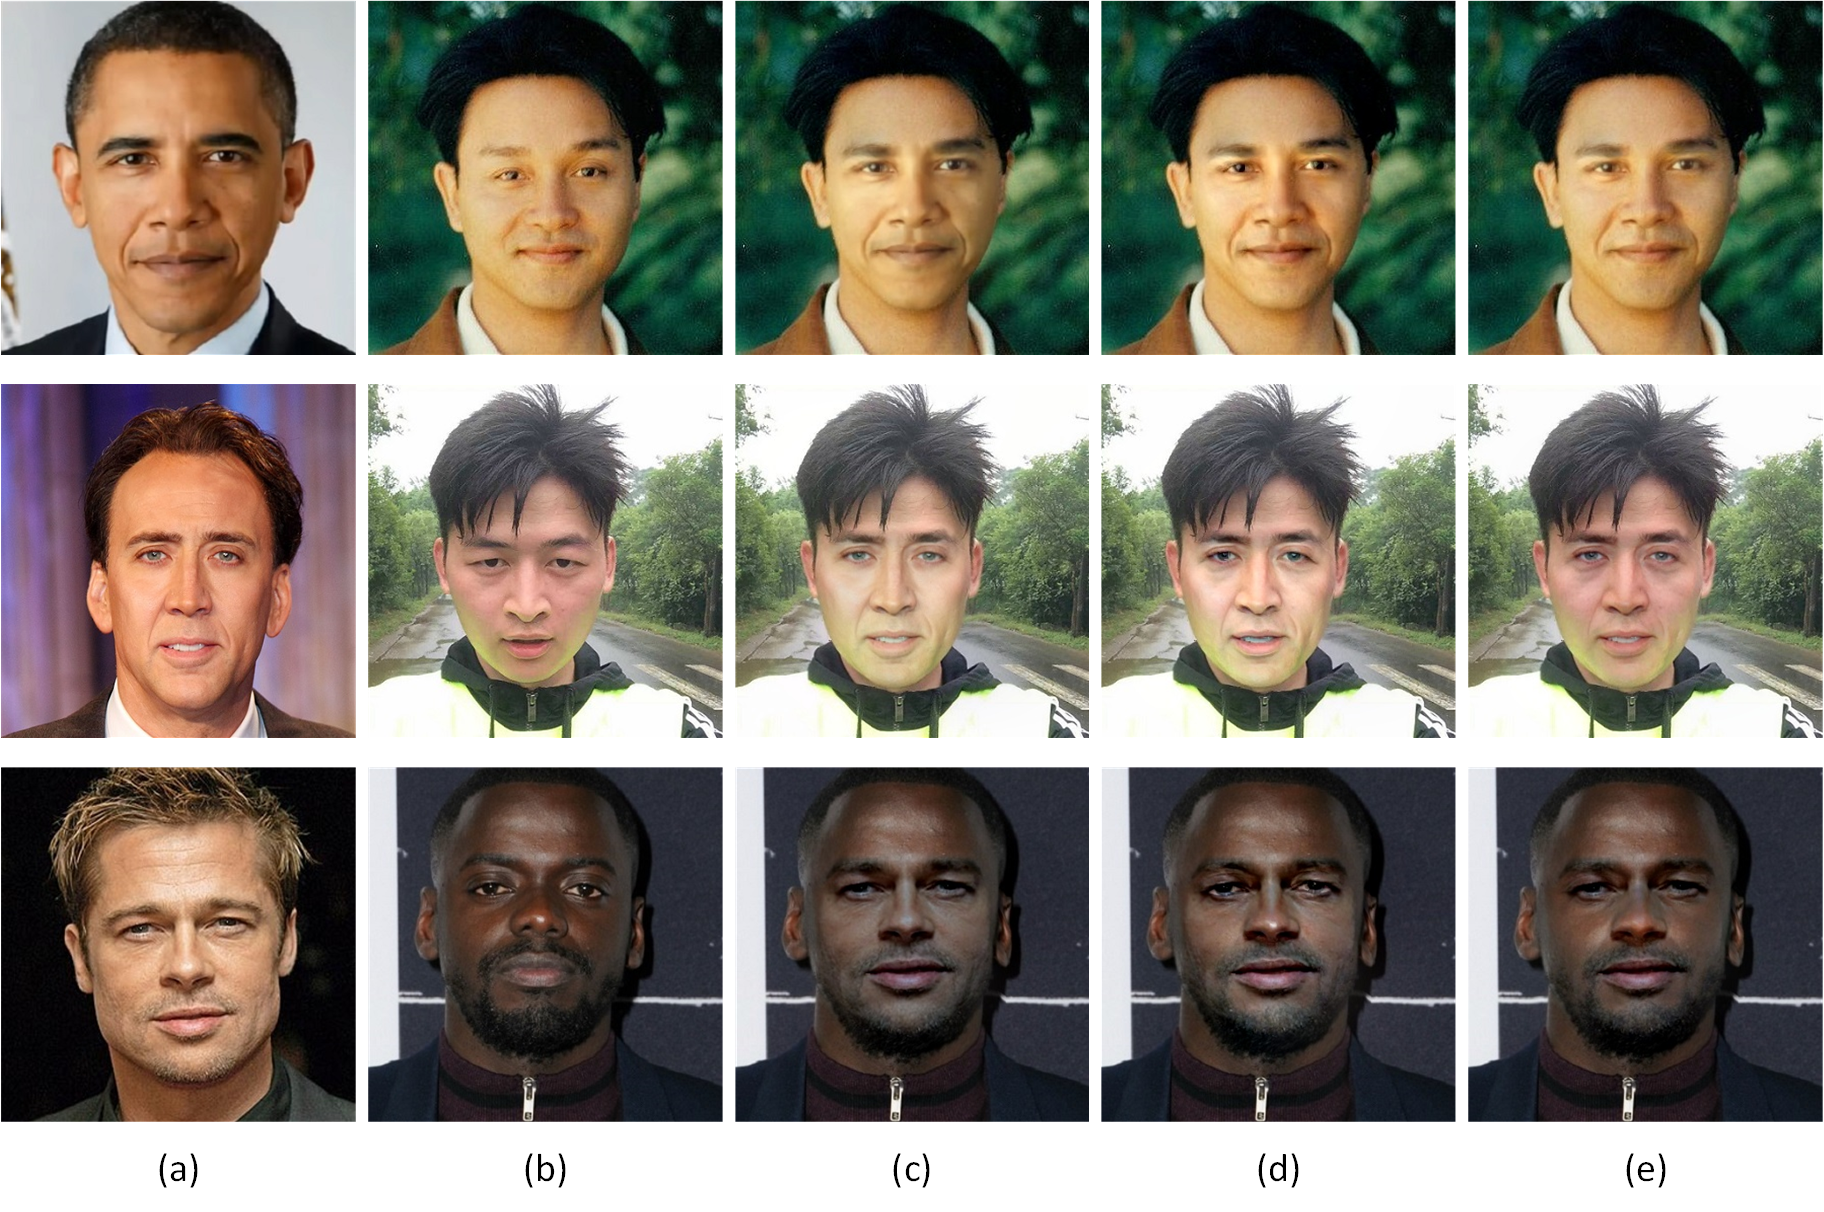
\includegraphics[width=4.8in]{images/3cmp.png}
    \fcaption{The effects of different gradient reconstruction: (a) Source face image. (b) Target face image. (c) Fusing face by linearly combining the gradients of two faces. (d) Fusing face by keeping the larger gradients of two faces. (e) Fusing face through weaker gradient preserving method.}
\end{center}

Fig. 4 shows the effects of different face gradient reconstruction. From Fig. 4(c), we can see that direct linear combination of  gradients of two faces could bring too much illumination from the source face into the target face, which makes face look very unnatural. If we kept the stronger gradients of two faces, the lightning condition of the target face would be strongly broken. More importantly, we can't control how much features we are going to fuse from the source face into the target face. In Fig. 4(e), the lightning condition and facial hues is closest to the target face image among all the results. When we reconstruct gradients using the proposed algorithm, we only keep the stronger gradients of the source face, which means the main features of the source are preserved.

\subsection{How the different parameters effect face fusion}
 For our task, there are four parameters we can adjust, they are $\alpha$, $\beta$, $\theta_1$, $\theta_2$. $\alpha$ controls the structure of human faces, in other words, it controls the profile and the distribution of features of human faces. $\beta$ controls the details of human faces, like wrinkles and textures. With $\alpha$ and $\beta$, we can control how much content we want to fuse from source face into target face. If the gradients of source face is weaker than $\theta_1$ and the gradients of target face is weaker than $\theta_2$, then we retain the gradients of the target face. Otherwise, we keep the gradients of the source face.

Fig. 5 shows how $\alpha$ effects the fused results, $\beta = 0.5$, $\theta_1 = 10$, $\theta_2 = 15$. As the $\alpha$ grows bigger, the distribution of face features of fused face is more like the source face.

\begin{center}
    \includegraphics[width=4.8in]{images/pro.png}
    \fcaption{(a) Source face. (b) Target face. (c) Fused face, $\alpha = 0.2$. (d) Fused face, $\alpha = 0.4$. (e) Fused face, $\alpha = 0.6$. (f) Fused face, $\alpha = 0.8$.}
\end{center}

Fig. 6 shows how $\beta$ effects the fused result. $\alpha = 0.5$, $\theta_1 = 10$, $\theta_2 = 15$. As the $\beta$ grows bigger, the fused result has more details from source face.

\begin{center}
    \includegraphics[width=4.8in]{images/detail.png}
    \fcaption{(a) Source face. (b) Target face. (c) Fused face, $\beta = 0.2$. (d) Fused face, $\beta = 0.4$. (e) Fused face, $\beta = 0.6$. (f) Fused face, $\beta = 0.8$.}
\end{center}

If we want to only keep main features of source face, we could only retain stronger gradients of the source face, Fig. 7 shows that the fused results are more natural as more weaker gradients of the source face are been dropped. $\alpha = 0.5$, $\beta = 0.5$, $\theta_2 = 40$. The weaker gradients carry too much illumination information and facial hues of the source face, when these gradients are brought into the fused results, the results become very unnatural.

\begin{center}
    \includegraphics[width=4.8in]{images/thd1.png}
    \fcaption{(a) Source face. (b) Target face. (c) Fused face, $\theta_1 = 2$. (d) Fused face, $\theta_1 = 4$. (e) Fused face, $\theta_1 = 6$. (f) Fused face, $\theta_1 = 8$.}
\end{center}

When we fuse the main features of source face into target face, somehow, we need to erase the main features of target face. In fact, we want to keep the illumination information of the target face, both the weaker gradients of source face and weaker gradients of target face are preserved. For Fig. 8, it shows the experiment on $\theta_2$,  $\alpha = 0.5$, $\beta = 0.5$, $\theta_1 = 10$, when the $\theta_2$ grows bigger, more stronger gradients are preserved. As we can see, more shadows are preserved.

\begin{center}
    \includegraphics[width=4.8in]{images/thd2.png}
    \fcaption{(a) Source face. (b) Target face. (c) Fused face, $\theta_2 = 10$. (d) Fused face, $\theta_2 = 20$. (e) Fused face, $\theta_2 = 30$. (f) Fused face, $\theta_2 = 40$.}
\end{center}

Although our work are not aiming at face swapping task, we still could create similar effects by setting $\beta = 1$. This means we almost preserving all the gradients of source faces, but only keep part of weaker gradients of target faces. We compare our results and the work of Korshunova et al. \cite{faceswapping}. In Fig. 9, the source face of all the results is from Fig. 8(a), we can see that our results keep more illumination information and facial hues of target faces which makes our results more natural. But in Fig. 9(c), our result fail to catch the lightning condition of the target face from a high level, this is where we need improve.

\begin{center}
    \includegraphics[width=4.8in]{images/vs.png}
    \fcaption{The first row are the original target face, the second row are the results of Korshunova et al., the third row are our results. Our algorithm preserves more illumination information and facial hues of target face.}
\end{center}

In Fig. 10, as $\alpha$ and $\beta$ grow bigger, the output face has more features from the source face.

\begin{center}
    \includegraphics[width=4.8in]{images/trans.png}
    \fcaption{(a) Source face. (b) Target face. (c) Fused face, $\alpha = 0.2$, $\beta = 0.2$. (d) Fused face, $\alpha = 0.4$, $\beta = 0.4$. (e) Fused face, $\alpha = 0.6$, $\beta = 0.6$. (f) Fused face, $\alpha = 0.8$, $\beta = 0.8$. (g) Fused face, $\alpha = 1$, $\beta = 1$.}
\end{center}

\section{Conclusions}

We developed a face fusion method that automatically fuses features of source face into target face. When we consider fusing human faces, there are two parts we are going to fuse, one is face structures, the other is face details. The 68 facial landmarks are enough to align two faces precisely. The illumination of source face might pollute target face. But the method we proposed preserves as much illumination information as possible while decreasing the influence of the illumination of the source face. At mean time, we developed a user interface for letting users control how many features they want from the source face to fuse into the target face. The limitation of our method is clear, we have small tolerance to pose variation. Once two faces are in different poses, warping faces changes the original distributions of face features.
\begin{thebibliography}{4}

\bibitem{fbim} Beier, T., Neely, S.: Feature-based image metamorphosis. In: ACM SIGGRAPH Computer Graphics, Vol. 26, No. 2, pp. 35-42 (1992)
\bibitem{autorep}Bitouk, D., Kumar, N., Dhillon, S., Belhumeur, P., Nayar, S. K.: Face swapping: automatically replacing faces in photographs. ACM Transactions on Graphics (TOG), 27(3), 39. (2008)
\bibitem{exchface}Blanz, V., Scherbaum, K., Vetter, T., Seidel, H. P.: Exchanging faces in images. In: Computer Graphics Forum, Vol. 23, No. 3, pp. 669-676 (2004)
\bibitem{fld4}Cao, X., Wei, Y., Wen, F., Sun, J.: Face alignment by explicit shape regression. In: International Journal of Computer Vision. (2014)
\bibitem{de1}De La Hunty, M., Asthana, A., Goecke, R.: Linear facial expression transfer with active appearance models. In: International Conference on Pattern Recognition (ICPR) (2010)
\bibitem{fld}Kazemi, V., Sullivan, J.: One millisecond face alignment with an ensemble of regression trees. In: Proc. IEEE Conf. Computer Vision and Pattern Recognition (CVPR), pp. 1867-1874 (2014)
\bibitem{mhf}Karungaru, S., Fukumi, M., Akamatsu, N.: Morphing Human Faces: Automatic Control Points Selection And Color Transition. In: International Conference on Computational Intelligence, pp. 224-227 (2004)
\bibitem{faceswapping}Korshunova, I., Shi, W., Dambre, J., Theis, L.: Fast face-swap using convolutional neural networks. arXiv preprint arXiv:1611.09577. (2016)
\bibitem{3d1}Lin, Y., Lin, Q., Tang, F., Wang, S.: Face replacement with large-pose differences. In: Proceedings of the 20th ACM international conference on Multimedia. (2012)
\bibitem{de3}Lin, Y., Wang, S., Lin, Q., Tang, F.: Face swapping under large pose variations: A 3D model based approach. In: International Conference on Multimedia and Expo (ICME), pp. 333-338 (2012)
\bibitem{de4}Mosaddegh, S., Simon, L., Jurie, F.: Photorealistic Face de-Identification by Aggregating Donors�� Face Components. In: Asian Conference on Computer Vision, pp. 159-174 (2014)

\bibitem{onseg}Nirkin, Y., Masi, I., Tran, A. T., Hassner, T., Medioni, G.: On Face Segmentation, Face Swapping, and Face Perception. arXiv preprint arXiv:1704.06729. (2017)
\bibitem{pie}P��rez, P., Gangnet, M., Blake, A.: Poisson image editing. In: ACM Transactions on Graphics (TOG), Vol. 22, No. 3, pp. 313-318 (2003)


\bibitem{fld3}Ren, S., Cao, X., Wei, Y., Sun, J.: Face alignment at 3000 fps via regressing local binary features. In: Proceedings of the IEEE Conference on Computer Vision and Pattern Recognition.(2014).
\bibitem{de2}Ross, A., Othman, A.: Visual cryptography for biometric privacy. In: IEEE transactions on information forensics and security.(2011)


\bibitem{wol}Wolberg, G.: Image morphing: a survey. In: The visual computer, 14(8), 360-372 (1998)



\bibitem{fld2}Xiong, X., De la Torre, F.: Supervised descent method and its applications to face alignment. In: Proceedings of the IEEE conference on computer vision and pattern recognition.(2013)





\end{thebibliography}



\end{document}
